\documentclass{article}
\usepackage[T1]{fontenc}
\usepackage[utf8]{inputenc}
\usepackage{graphicx}
\usepackage{verbatim}
\usepackage{geometry}
\usepackage[french]{babel}

\geometry{hmargin=2.5cm,vmargin=2cm}
\usepackage{xcolor}


\definecolor{codegreen}{rgb}{0,0.6,0}
\definecolor{codegray}{rgb}{0.5,0.5,0.5}
\definecolor{codepurple}{rgb}{0.58,0,0.82}
\definecolor{backcolour}{rgb}{0.95,0.95,0.92}

\usepackage[final]{listings}
\lstdefinestyle{code}{
  belowcaptionskip=1\baselineskip,
  breaklines=true,
  frame=L,
  xleftmargin=\parindent,
  language=C,
  showstringspaces=false,
  basicstyle=\footnotesize\ttfamily,
  keywordstyle=\bfseries\color{green!40!black},
  commentstyle=\itshape\color{purple!40!black},
  identifierstyle=\color{blue},
  stringstyle=\color{orange},
}
\lstset{style=code, language=C}

\usepackage{hyperref} % Créer des liens et des signets
\hypersetup{
colorlinks = true, %colorise les liens
breaklinks = true, %permet le retour à la ligne dans les liens trop long
urlcolor = blue, %couleur des hyperliens
linkcolor = blue, %couleur des liens internes
citecolor = black, %couleur des références
frenchlinks = true
}

\begin{document}

\begin{titlepage}
    \centering
    \Huge\bfseries
    Implémentation du Splendor en C

    \begin{center}
    
\includegraphics[scale=2]{enseirb.png}
    \centering
    \end{center}
    
    \vspace{5cm}

    \Large
    Romane CAVEY, Constantin PALLUAT
    
    \vspace{1cm} 
    
    
    \Large
    ENSEIRB-MATMECA 2023-2024
    
    \vspace{0.5cm} 

    
    \vfill % Remplissage de l'espace vertical restant
    
   
\end{titlepage}

\tableofcontents

\newpage

\section{Introduction}

\hspace{1em} Le projet que nous avons réalisé repose sur l'implémentation d'une copie simplifiée du jeu de société "Splendor". 

\vspace{1em} Dans cette version le joueur doit acquérir le maximum de points de prestige en achetant des architectes à l'aide de jetons représentant des ressources. Chaque joueur possède une action par tour: acheter un architecte ou piocher une pièce. Ce jeu demande donc au joueur une bonne gestion de ses cartes afin de construire un moteur économique efficace.

% Insérer schéma descriptif du jeu ?

    \subsection{Objectifs}
    \hspace{1em} Ce projet dispose d'objectif à la fois théoriques et pratiques permettant de développer un ensemble de compétences techniques mais aussi humaines.
    
        \subsubsection{Objectifs théoriques}
        \hspace{1em} Les objectifs théoriques ont pour but de faire évoluer nos aptitudes de programmation. Voici donc une énumération de ceux ci:

        \begin{itemize}
            
            \item Apprendre à organiser un projet contenant une multitude de fonctionnalités
            \item Apprendre à gérer les dépendances
            \item Mieux s'approprier les outils et concepts de base du language C
            \item Améliorer nos techniques de débogage
        \end{itemize}
    
        \subsubsection{Objectifs pratiques} 
        \hspace{1em} En pratique, ce projet est le fruit du travail d'un binôme et nous permet d'améliorer nos compétences de communication, d'écoute, d'organisation et de gestion en général.
        
        \vspace{1em} De plus, ce projet nous met faces aux impératifs que représentent les délais de rendu et la satisfaction des consignes.

   
    \subsection{Cahier des charges}[!ht]
    \hspace{1em} Voici le cahier des charges permettant de donner une première ébauche de l'articulation de notre projet: 
        \begin{table}[h]
        \centering
        \begin{tabular}{|c|p{5cm}|p{8cm}|}
            \hline
            \textbf{ID} & \textbf{Besoins} & \textbf{Implémentations} \\
            \hline
            2.2 & Retranscrire les différentes entités du jeu  & Créer des structures et fonctions adaptées \\
            \hline
            2.3 & Pouvoir piocher une pièce & Créer des fonctions de modifications de la main du joueur et du marché\\
            \hline
            2.3 & Pouvoir acheter un architecte & Créer des fonctions de vérifications de coût et de modification de la guilde\\
            \hline
            3 & Création de parties aléatoires & Mettre en place une boucle de jeu de parties aléatoires affichant le vainqueur ainsi que son nombre de points \\
            \hline
        \end{tabular}
        \caption{Cahier des charges de la version simplifiée du jeu}
        \label{table:cahier_des_charges}
\end{table}
\section{Implémentation}

\hspace{1em} Dans cette section, nous allons expliquer comment nous avons retranscrit le jeu sous forme d'instructions machines tout en justifiant nos choix de conception. \textbf{Nous allons donc détailler uniquement les structures et solutions algorithmiques que nous avons été amené à écrire par notre propre chef et non celles déjà données dans le sujet en considérant que celles-ci sont acquises par le lecteur.}

    \subsection{Organisation des fichiers}
    \hspace{1em} Nous avons regroupé nos fichiers nécessaires pour notre projet dans le dossier "src" et nos tests dans le dossier "tst". L'avancement du projet et le renouvellement récurrent des fonctions déjà écrites nous a montré à quel point il était important de bien scinder son projet en plusieurs fichiers afin d'éviter les problèmes de dépendance.
    
    \vspace{1em} Ainsi, nous avons décidé de créer un fichier pour chaque entité du jeu (marché, guilde, jetons, architectes), pour chaque nouvelles fonctionnalités (faveurs, super architectes) et pour les fonctions du jeux en général comme l'illustre la figure 1.
    
    \newpage




\begin{lstlisting}[frame=single, caption={Organisation et arborescence de nos fichiers},label=organisation]
    Makefile
    project
    README.md
    src
        ansi_color.h
        builder.c
        builder.h
        builder_set.c
        color.c
        color.h
        favor.c
        favor.h
        game.c
        game.h
        guild.c
        guild.h
        market.c
        market.h
        permutation.c
        permutation.h
        player.c
        player.h
        power.c
        power.h
        project.c
        project.o
        second_builder.c
        second_builder.h
        second_color.h
        second_token.c
        second_token.h
        set.c
        set.h
        stack.c
        stack.h
        super_builder.c
        super_builder.h
        super_token.c
        super_token.h
        token.c
        token.h
    tst
        test_achiev1.c
         test_achiev1.h
        test_achiev2.c
        test_achiev2.h
        test_achiev3.c
        test_achiev3.h
        test.c
        test.h
        test_init.c
        test_init.h
        test_main_achiev2.c
        test_main.c



\end{lstlisting}

        
    \vspace{3em} On peut noter que le sujet nous imposait de travailler avec des fichiers de base tel que builder.*, token.* et color.* dans lesquels on ne pouvait pas rajouter de fonctions et que lors de l'écriture de notre code nous avons jugé qu'il était bon de rajouter des fonctions liées au builder et token. C'est pour cela que nous avons écrits des nouveaux fichiers avec le label "second" au début.

    Par ailleurs, nos fichiers sont assez dépendants les uns des autres comme l'illustre le listing \ref{orga}, nous avons même eu un problème de cycle d'inclusion des .h (cf section 5 Difficultés). 

    \begin{figure}
    \centering
    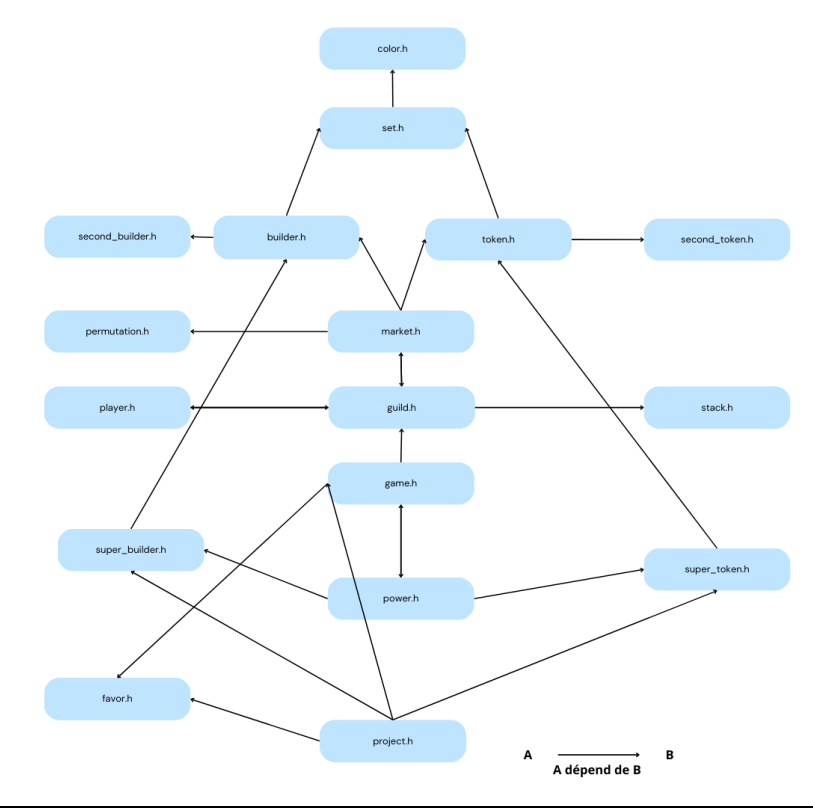
\includegraphics[scale=0.60]{dependance.png}
    \label{orga}

\end{figure}

    
    %IDEE: ON PEUT ENTOURER LES FICHIERS SECONDS EN ROUGE SUR LA FIGURE ?
    
    \subsection{Stucture et initialisation des différentes entités du jeu}
    \vspace{1em}
    \hspace{1em} Pour simplifier nos démarches sur la durée du projet, nous avons décidé de travailler exclusivement avec des pointeurs car les transferts de jetons et d'architectes entre les joueurs et le marché/la guilde impliquaient un changement récurrent de l'état des mains des joueurs tout en conservant les mêmes architectes et jetons qu'à l'initialisation du jeu.

    \hspace{1em} Nous avons également choisis de ne pas travailler en boîte noire pour implémenter nos entités (ex: la guilde et le marché) quand nous en avions la possibilité afin de pouvoir manipuler plus simplement les structures dans nos autres fichiers.

    %FAIRE LE GRAPHE DE DEPENDANCE COMME INDIQUE DANS LE MAIL

    %FAIRE SCHEMA DES GUILD ET MARCHER QUI POINTENT VERS + exliciter la façon dont ils sont initialisés
        \subsubsection{Les jetons et les architectes} 
        \hspace{1em} Au début du projet les structures des jetons et des architectes étaient imposés. Cependant, arrivé à l'achievement 2, le sujet nous demandait de factoriser notre code afin d'obtenir une structure similaire pour les deux entités à l'aide d'une structure commune "set\_t" décrite sur le listing \ref{struct_set}.

\begin{lstlisting}[language=c, frame=single, caption={Implementation de la structure set\_t},label=struct_set]
struct set_t {
    unsigned int ressource[NUM_COLORS];
 };

\end{lstlisting}
            
        \vspace{0.5cm}
        La structure \textbf{"set\_t"} contient un tableau d'entier qui permet de représenter les couleurs du jeu.

        Le listing \ref{struct_token} et \ref{struct_builder} montrent la manière dont nous avons factorisé notre code:
        \vspace{0.5cm}

\begin{lstlisting}[frame=single, caption={Code des structures des jetons },label=struct_token]
struct token_t {
  struct set_t s;
};
\end{lstlisting}

    \vspace{0.5cm}

\begin{lstlisting}[frame=single, caption={Code des structures des architectes},label=struct_builder]
struct builder_t{
    char level;
    int points;
    struct set_t ressource;
    struct set_t production;
};
\end{lstlisting}
\vspace{0.5cm}
        Cette factorisation permet de manipuler, dans la suite de notre projet, d'assimiler les structures des jetons à celles des architectes. 

        \vspace{1em} \textbf{Initialisation des architectes:} Le nombre total d'architectes en jeu est "MAX\_BUILDERS" (instruction pré-processeur), nous avons donc décidé de stocker tous les architectes du jeu dans un tableau que nous appelons \textbf{"game\_builders"} et défini dans le fichier "builder.c". Nous verrons par la suite comment à l'aide de ce tableau et de pointeurs nous pouvons initialiser la guilde et le marché.
        Le tableau est initialisé avec des structures nulles.
        Nous le modifions ensuite en place à l'aide d'une fonction \textbf{init\_builders} qui prend en paramètre une seed d'aléatoire. Nous avons décidé que le nombre de builder pouvait être inférieur à MAX\_BUILDERS fixé à 10 dans le jeu de base mais qu'il devait être supérieur ou égal à 5.
        Nous avons donc utilisé des modulos pour borner dans un intervalle des valeurs aléatoires comme par exemple:
        \begin{verbatim} nb_builders = 5 + (rand() % (MAX_BUILDERS - 5));
        \end{verbatim}
        
        Cette ligne permet de décider aléatoirement du nombre d'architectes que nous aurons réellement dans notre jeu par la suite. On aura au moins 5 architectes auquel on vient additionner une valeur aléatoire comprise entre 0 et MAX\_BUILDER-5 (le -5 sert à ne pas dépasser le nombre d'architectes maximal).

        Par des procédés similaires, une fois le nombre d'architectes décidé, on vient modifier aléatoirement les champs des structures des architectes compris dans le tableau. On obtient alors un tableau d'architectes initialisé aléatoirement. La figure \ref{init_builder} reprend l'explication à l'aide d'un exemple:

 
        \begin{figure}[!ht]
            \centering
            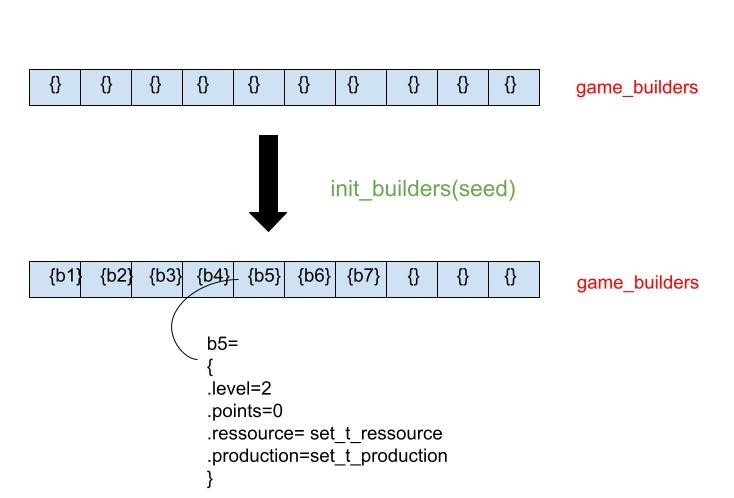
\includegraphics[width=0.7\linewidth]{Init builder.jpg}
            \caption{Exemple d'initialisation des architectes}
            \label{init_builder}
        \end{figure}

        
        \vspace{1cm}\textbf{Initialisation des jetons:} Les jetons sont initialisés de manière similaire dans un tableau \textbf{"all\_tockens"} défini dans le fichier "second\_token.c". La seule différence avec l'initialisation des architectes est que les jetons sont initialisées en nombre connu "NUM\_TOKENS" et qu'elle peuvent être complexes ou simples. Nous avons décidé qu'une pièce était complexe avec une probabilité de 50\%.
        
        \subsubsection{La guilde}

        \hspace{1em} Dans un premier temps, la guilde était simplement un espace permettant d'informer les joueurs de la disponibilité des architectes.
       Notre première approche pour l'implémentation des guildes était donc une structure contenant plusieurs champs représentés sur le listing \ref{struct_guild_achiev0}.  

   \vspace{1em}

        \begin{lstlisting}[frame=single, caption={Code de la structure de la guild pour de l'achievement 0},label={struct_guild_achiev0}]
struct guild_t{
    int nb_builder;
    struct builder_t* builder_in_guild[MAX_BUILDERS]; //All the builder of the guild
};

    \end{lstlisting}
   
   \vspace{1em}
        \textbf{Explication:} Cette structure contient un entier qui retranscrit le nombre d'architectes disponibles dans la guilde et un tableau de pointeurs vers les architectes de l'ensemble des architectes de la partie. Si l'architecte n'était plus disponible (après qu'un joueur l'ait choisi), le pointeur pointait vers NULL. La figure \ref{schema_guild} récapitule sont fonctionnement.

         
        \begin{figure}[!ht]
            \centering
            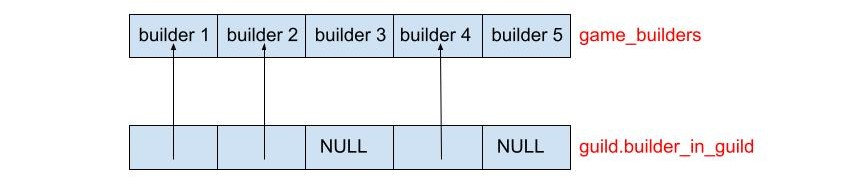
\includegraphics[width=\linewidth]{schema_guild.jpg}
            \caption{Schéma explicatif du principe de la guilde}
            \label{schema_guild}
        \end{figure}

        Nous avons choisi cette approche à l'aide de pointeurs afin de faciliter la comparaison entre les architectes: il est plus simple de comparer des adresses de structures que les structures en elles-mêmes.
    
        \vspace{1em} Dans la suite du projet (achievement 1), nous avons dû faire évoluer la guilde pour gérer les contraintes d'embauches des architectes imposées par le sujet. La guilde ne mettait à disposition, pour chaque niveau disponibles, qu'un certain nombre de builders (MAX\_BUILDERS\_AVAILABLE\_PER\_LVL) qui peuvent être embauchés à chaque tour. Nous avons donc modifié notre structure et utilisé une méthode se basant sur les piles( cf listing \ref{struct_guild}). 
        
        \vspace{1em}
        
         \begin{lstlisting}[frame=single, caption={Code de la structure de la guild pour de l'achievement 1},label=struct_guild]
struct guild_t{
    int nb_builder;
    struct builder_t* builders[MAX_BUILDERS]; //All the builder of the beginning
    struct builder_t* builder_available[MAX_BUILDERS];// The MAX_BUILDER_PER_LEVEL we can pick each turn
    struct stack_t stack[NUM_LEVELS];
};

    \end{lstlisting}
        \vspace{1em}

        \textbf{Explication:} Cette structure contient toujours l'entier nb\_builder qui décrit le nombre d'architectes disponibles dans la guilde: ceux visibles pour les joueurs et ceux en stock. 
        2 autres des champs sont des tableau de pointeurs de taille (MAX\_BUILDERS) vers des structures d'architectes. Le tableau \textbf{"builder"} sert à l'initialisation et nous expliciteront son rôle par la suite. Le tableau \textbf{"builder\_available"} possède des pointeurs vers les architectes que les joueurs peuvent prendre lors de leur tour.
        Le dernier champ est un tableau de structure de pile; structure que nous avons écrit comme on peut le voir sur la figure \ref{struct_stack}
        
        \vspace{1cm}

        \begin{lstlisting}[frame=single, caption={Code de la structure "stack\_t"},label={struct_stack}]
struct stack_t{
    int nb;
    int head;
    struct builder_t* values[2*MAX_BUILDERS];
};

    \end{lstlisting}


        On retrouve une structure classique de pile manipulable à l'aide d'un tableau et des entiers \textbf{"nb"} et \textbf{"head} qui donnent respectivement le nombre d'élément dans la pile et l'indice de la tête de pile. La pile permet de stocker des pointeurs d'architectes.

        \vspace{1em}
        
        \textbf{Principe de mise à disposition des architectes pour les joueurs:}
        Lorsque qu'un joueur prend un architecte dans la guilde, le pointeur du tableau \textbf{"builder\_available"} se met à NULL puis on vient remplacer cet architecte par un architecte de niveau semblable si on le peut. On remplace alors ce pointeur par la tête de la pile correspondant au niveau de l'architecte choisi. Si la pile est vide on regarde dans les piles d'autres niveau jusqu'à atteindre une pile non vide ou alors après avoir parcouru l'ensemble des piles. La figure \ref{explication_guild_achiev1} récapitule l'explication avec un exemple:

 
        \begin{figure}[!ht]
            \centering
            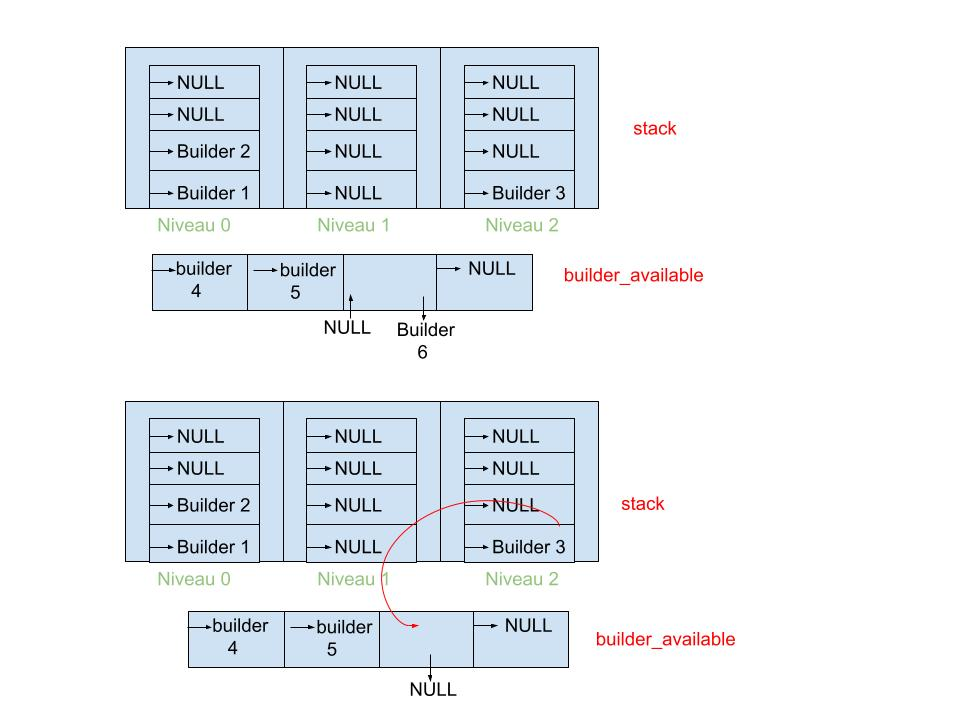
\includegraphics[width=0.7\linewidth]{explication_guild_achiev1.jpg}
            \caption{Exemple explicatif de la mise à disposition des architectes}
            \label{explication_guild_achiev1}
        \end{figure}

        \vspace{1cm}
        
        Ici, on considère que le \textbf{builder 6} est de niveau 1. Le joueur choisi l'architecte 6 dans ceux qui sont mis à disposition. On met donc le pointeur vers l'architecte 6 à "NULL". On cherche ensuite un architecte dans la pile de niveau 1 qui est vide, on passe alors à la pile d'après (pile de niveau 2) dont la tête est un pointeur vers l'architecte 3. On remplace le pointeur du tableau builder\_available par le pointeur vers l'architecte 3 et on met le pointeur de la pile à NULL.

        \vspace{1em}
        
        \textbf{Justification de ce choix d'implémentation}: Cette implémentation à l'aide de pile permet d'alléger la complexité de nos programmes. En effet, le remplacement d'un architecte pris précédemment requiert une recherche dans les différentes piles or, ici,la complexité est constante grâce aux indices de tête qui permettent d'éviter une recherche itérative dans un tableau (dont la recherche est de complexité linéaire).

        \vspace{1em} \textbf{Initialisation:} La première version de notre guilde était initialisée très facilement, nous devions juste faire pointer ses éléments vers les éléments de notre tableau d'architectes "game\_builders".
        
        L'ajout du système de pile a complexifié la manière d'initialiser notre guilde. Le tableau \textbf{"builders"} pointe vers "game\_builders" puis, à l'aide d'une double boucle nous rangeons l'ensemble des pointeurs de ce tableau par niveau dans leurs piles respectives. On vient ensuite, encore une fois à l'aide d'une double boucle, parcourir chaque pile de niveau et mettre "MAX\_BUILDERS\_AVAILABLE\_PER\_LVL" (ou moins si nous n'avons pas assez d'architectes dans cette tranche de niveau)  dans le tableau \textbf{"builder\_available"}.
        %REMPLIIIIR ICIIIIIII
        \subsubsection{Le marché} Dans un premier temps, à l'image de la guilde, la marché était un endroit permettant de mettre à disposition les jetons pour les joueurs. Nous l'avons donc modélisé selon le même principe:


\begin{lstlisting}[frame=single, caption={Code la structure de notre marché},label={struct_market_achiev0}]
struct market_t{
    int nbr_token;
    struct token_t* available_tokens[NUM_TOKENS];
};

    \end{lstlisting}
      

        Cette structure contient le nombre de jetons dans le marché et un tableau de pointeurs vers les jetons du jeu. Cette implémentation contient exactement les mêmes avantages que pour la guilde.

        Par la suite, comme pour la guilde, le marché a évolué selon les consignes du sujet. Le marché est considéré comme un plateau avec un sens de parcours où les joueurs peuvent piocher les jetons connexes à la case sur laquelle ils se trouvent dans le marché. Nous avons alors changé notre structure comme on peut le voir sur la figure \ref{struct_market_achiev1}


        \begin{lstlisting}[frame=single, caption={Modification de la structure de notre marché pour l'achievement 1},label={struct_market_achiev1}]
struct market_t{
    int nbr_token;
    struct token_t* playing_board[NUM_TOKENS];
    int permutation[NUM_TOKENS];
};

    \end{lstlisting}
      



        Les changements notables au sein de la structure sont le tableau de permutation dont nous allons expliciter l'utilité par la suite. Malgré que la structure ai très peu changée, le principe de fonctionnement du marché à bien évolué. On dispose maintenant d'un plateau de jeu, et on dispose les jetons selon une permutation ,qu'on considère donnée (sous forme de cycle). Pour piocher des jetons, il faut que celles-ci soit connexes sur le plateau , on a donc un tableau de jeu de taille NUM\_TOKENS qui modélise ce plateau.

            De même, pour remettre les jetons, on les remet à la première place vide du plateau.
        
        
        
        \subsubsection{Les joueurs} %interet du tableau= multiplayer facile%

        Nous avons implémenté les joueurs par ce qu'ils pouvaient posséder: des points de victoire, des architectes et des jetons.
        La structure des joueurs n'a que très peu évolué au cours du projet et a conservé quasiment le même fonctionnement. Le listing  \ref{struct_player_achiev0} montre cette structure:

        \vspace{1em}

 \begin{lstlisting}[frame=single, caption={Structure d'un joueur},label={struct_player_achiev0}]
struct player{
    struct token_t* player_token[NUM_TOKENS];
    struct builder_t* player_builder[MAX_BUILDERS];
    int points;
    int nbr_token;
    int nbr_builder;
    int index;
    int favor_nbr;
};

    \end{lstlisting}
    \vspace{1em}      

        De la même manière que pour la guilde ou pour le marché, les possessions des joueurs sont représentés à l'aide de tableaux de pointeurs (vers des architectes ou des jetons) et des entiers décrivant leur nombre. Naturellement, le nombre de points de victoire est retranscrit à l'aide d'un entier \textbf{"points"}.\\
        Enfin, l'entier \textbf{"index"} sert d'identificateur. En effet, dès le début du projet nous avions imaginé notre code de manière à ce qu'il fonctionne pour des parties de plus de 2 joueurs et nos joueurs sont initialisés dans un tableau de taille "NB\_PLAYERS". L'entier \textbf{"index"} correspond alors à l'index du joueur dans ce tableau.


        \textbf{Initialisation des joueurs:} L'initialisation se fait simplement avec des structures vides lors de la création du tableau "players".

        
        \subsubsection{Pouvoirs et faveurs}
            \textbf{Les pouvoirs:} Pour implémenter les pouvoirs, nous avons dû implémenter un nouveau type à l'aide d'un typedef. Tout d'abord, on créer un enum des pouvoirs comme le montre le listing \ref{enum_pouvoir} suivant:

             \begin{lstlisting}[frame=single, caption={Enum des pouvoirs },label=enum_pouvoir]
            enum power_id{
    PANIC_MARKET,
    PANIC_GUILD,
    TOKEN_STEAL,
    TURN_STOLEN,
    MASTER_HAND,
	GAIN_FAVOR_WITH_BUILDER,
	FAVOR_STEAL,
};
    \end{lstlisting}
    
    On a créé les fonctions qui correspondent aux pouvoirs , dans le power.c , comme guild\_renew, qui renouvelle la guild.
On a ensuite une fonction qui associe cet énum à la fonction du pouvoir associé. On utilise un typedef pour pouvoir créée un tableau de pouvoir "skill". Ces fonctions doivent avoir le même type donc prendre les mêmes paramètres et renvoyer la même valeur de retour. Ainsi ces fonctions prennent en argument le marché, la guild, le tableau des joueurs, l'indice du joueur actuel, et un élément void*. L'intérêt de cet élément de type void* est de pouvoir passer en paramètre un architecte ou un jeton, sans que cela soit défini au préalable, et de le caster dans le code comme tel. De même pour la valeur de retour, en réalité une seule fonction nécessite de renvoyer un entier ("turn\_stolen"), les autres pourraient être de type void, mais pour pouvoir créer ce typedef, on fait en sorte que tous les pouvoirs renvoient un entier.
\begin{lstlisting}[frame=single, caption={Implementation des pouvoirs },label=implementation_pouvoir]
            typedef int (*skill)(int current_player, struct player players[NB_PLAYERS], void* ressource,struct market_t *market,struct guild_t *guild);


            skill skills[NUM_POWER]={
	panic_market,
	guild_panic,
	token_steal,
	steal_turn,
	master_hand,
	gain_favor_with_builder,
	favor_steal
	
};
    \end{lstlisting}

 \vspace{1cm}

    Les pouvoirs ont également impacté la façon de considérer nos architectes et nos jetons. En effet , nous avons dû adapté notre structure pour que chaque élément (architecte et jeton) soit associé à un pouvoir. Pour ne pas avoir à changer toute l'implémentation de toutes nos fonctions, on décide de créer de nouvelles structures: 
\begin{lstlisting}[frame=single, caption={Implementation des supers\_builder },label=builder_power]

    struct builder_power{
	   struct builder_t* builder;
	   skill powers[NUM_POWER];
};
    \end{lstlisting}

\begin{lstlisting}[frame=single, caption={Implementation des supers\_tokens },label=token_power]

 struct token_power{
	struct token_t* token;
	skill powers [NUM_POWER];
};

    \end{lstlisting}

            
            \textbf{Les faveurs:} Cette fonctionnalité n'a modifier que très peu la structure globale de notre code, nous avons simplement rajouté des fonctions relatives aux faveurs. Le seul point notable est l'ajout d'un entier décrivant le nombre de faveur que possède le joueur dans la structure \textbf{"player"}. Les faveurs étaient alors utilisée dans la boucle comme nous allons le voir dans le partie 3.
            Nous allons seulement expliciter les fonctions qui retranscrivent les différentes faveurs. \\
            \textbf{Renouvellement de la guilde:} Les joueurs peuvent renouveler les architectes d'un même niveau dans la guilde. Le principe est simple, on recherche les architectes du niveau choisi dans le tableau \textbf{builders\_available} de la guilde puis on vient les stocker dans un tableau dédié. On vient ensuite regarder dans la pile du niveau choisi si il y assez d'architectes pour remplacer les anciens: si oui on "pop" les élement de la pile pour les mettre dans le tableau "builder\_available" sinon on vient combler les architectes restants en remettant ceux que l'on avait enlevé à la base. La figure \ref{favor_guild_renew} présente un exemple :
            
             
        \begin{figure}[!ht]
            \centering
            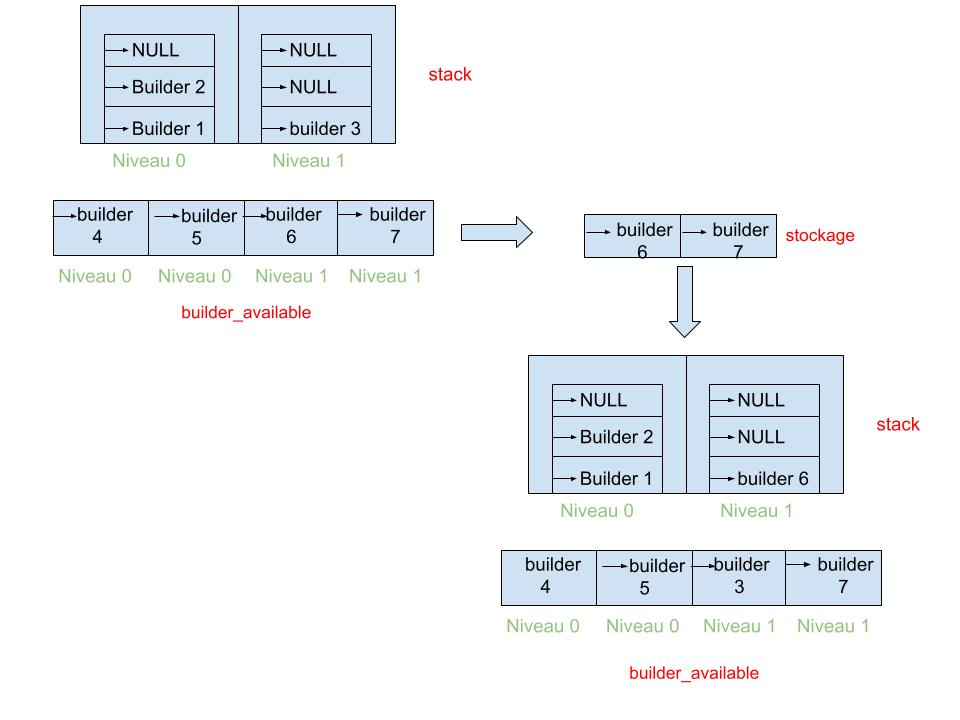
\includegraphics[width=0.8\linewidth]{favor_guild_renew.jpg}
            \caption{Exemple explicatif du renouvellement des guildes par les faveurs}
            \label{favor_guild_renew}
        \end{figure}

        \vspace{1cm}


        Ici, le joueur veut remplacer les architectes de niveau 1, la pile ne contenant qu'un seul builder, la guilde ne renouvelle qu'un seul architecte sur deux.

        Nous utilisons pleinement le potentiel des piles afin de simplifier les intéractions entre les architectes visibles et ceux en stock.

        \textbf{Choix d'une pièce dans le marché:} Le joueur peut aussi choisir la pièce qu'il veut dans le marché, qu'importe sa configuration à l'aide d'une faveur. La fonction ressemble aux fonctions écrites précédemment, nous avons seulement décidé que le joueur, étant la machine, choisissait une pièce au hasard dans le marché lors de l'exécution de la fonction.

    
    \subsection{Interaction entre les différentes entités du jeu}

    \subsubsection{Piocher des jetons dans le marché} Dans un premier temps la prise de jeton dans le marché se faisait simplement avec une redirection de pointeur. On parcourt le tableau contenant l'ensemble des pièces du joueur jusqu'à obtenir un pointeur "NULL", on le remplace par l'adresse du jeton choisi et on met le pointeur marché à "NULL".

    Dans un second temps, avec le problème de parcourt et de connexité des jetons dans le marché nous devions adapter notre approche. Nous avons donc codé une fonction permettant d'identifier les jetons connexes à un jeton contenu dans le marché. La figure \ref{jetons_connexes} montre un exemple de la connexité avec un exemple de plateau du jeu.

             
        \begin{figure}[!ht]
            \centering
            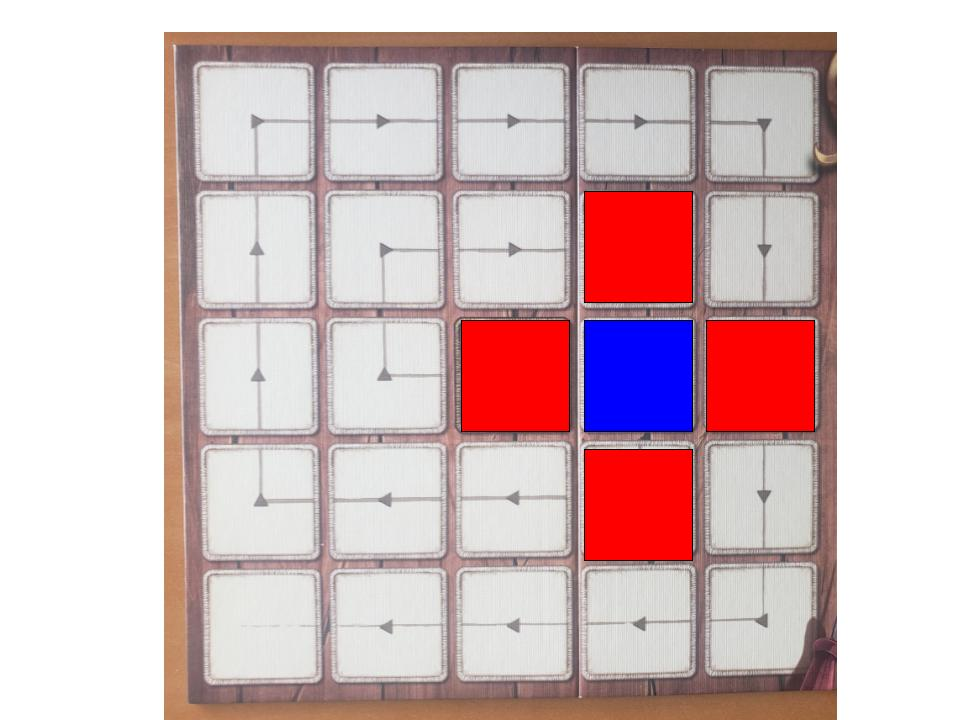
\includegraphics[width=0.4\linewidth]{jetons_connexes.jpg}
            \caption{Plateau du marché montrant la connexité des jetons}
            \label{jetons_connexes}
        \end{figure}
    
    Ici, la case bleue représente la case sur laquelle se situe l'avancement du plateau et les cases rouges représentent les jetons que l'on peut piocher. Nous avons une fonction qui détermine le nombre de jetons connexes d'un jeton donné ("token\_neighbour"). Une fois ce nombre connu, on appelle une autre fonction("token\_connex"), qui enlève le jeton du marché et le rajoute au compte du joueur grâce à la fonction "pick\_token", et fait de même pour le jeton du bas, du haut , à droite , puis à gauche, tant que le nombre de jetons choisis est inférieur au nombre de jetons à piocher.  On pose ligne=sqrt(NUM\_TOKENS) et on vérifie que les cases suivantes sont libres, auxquels cas, on les pioche : playing\_board[i], playing\_board[i+ligne], playing\_board[i-ligne], playing\_board[i+1], playing\_board[i-1], sans oublier de vérifier les bords, qui sont des cas particuliers.
    

    
    
    \subsubsection{Acheter des architectes} De tout notre projet, cette fonctionnalité a été l'une des plus difficile à écrire. Cette fonction est nommée "token\_pay" et, à chaque appel, permet d'\textbf{acquérir l'architecte}, de \textbf{supprimer les jetons} qui ont servi à payer l'architecte et de les \textbf{remettre dans le marché}. Elle est donc divisée en sous fonctions qui permettent une meilleur lisibilité du code et de ne modifier que certaines sous fonctions lors de changement d'implémentation par exemple.     
    
    \vspace{1em}  Les sous fonctions permettant d'effectuer les points énoncés plus tôt consistent en une grande redirection de pointeurs en parcourant les différents tabeaux des structures et en comparant les différentes adresses des pointeurs. Par exemple il faut rediriger les pointeurs des jetons du joueur pour les mettre à "NULL" après l'achat, faire pointer le marché vers les jetons que nous avons utilisé pour payer pour les remettre en circulation, faire pointer une des cases du tableau contenant les architectes vers l'architecte que nous avons choisi etc ...
    
    \vspace{1em} Avant de payer l'architecte il est important de savoir si le joueur a la capacité de l'acheter à l'aide des ressources qu'il dispose et de ce que les architectes produisent. Nous avons donc écrit une fonction pour effectuer ce test. Nous avions configuré, au départ, notre fonction afin qu'elle puise dire si le joueur pouvait payer exactement le coût d'embauche. Au début du projet, les architectes avait des coûts d'embauche unicolore. Nous avions alors deux compteurs: l'un qui calculait naïvement le nombre de ressources requis pour l'embauche sur chaque jetons du joueur et un autre compteur plus élaboré qui calculait le nombre de ressources requis uniquement sur les jetons simples ou complexe contenant 2 fois la même ressource. A la fin nous regardions si le compteur élaboré était supérieur au coût d'embauche, si oui on pouvait payer exactement, si non on regardait si le compteur naïf était supérieur pour déterminer si on pouvait payer ou non l'architecte. A noter que nous regardions d'abord si le joueur pouvait payer le coût d'embauche avec les ressources fournies par ses architectes avant de regarder ses jetons.
    La figure \ref{token_pay1} donne un exemple de cette fonction:

        \begin{figure}[!ht]
            \centering
            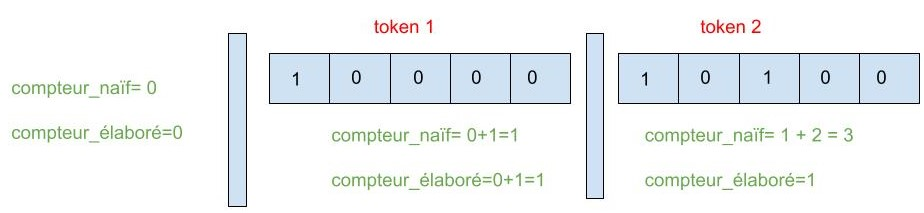
\includegraphics[width=0.7\linewidth]{token_pay1.jpg}
            \caption{Exemple de la fonction "token\_pay"}
            \label{token_pay1}
        \end{figure}

\vspace{2cm}

    On suppose ici que le joueur possède seulement deux jetons. Le compteur naïf ne fait pas la différence entre les deux jetons tandis que le compteur élaboré ne compte pas les ressources du deuxième jeton car il y aura une perte à la fin.
    
    \vspace{1em} Par la suite, avec la factorisation du code entre les architectes et les jetons, les coûts d'embauches étaient eux aussi multicolores. Les solutions algorithmiques de coût exact étant très difficiles à écrire nous avons décidé d'abandonner le compteur élaboré et de reprendre le même principe que précédemment avec des compteurs naïf sur chaque ressources de couleurs. Par exemple, même si cela n'est pas prévu dans le jeu, si l'architecte possède un coût d'embauche demandant 4 ressources différentes, nous allons utiliser 4 compteurs naïfs sur chacun des jetons du joueur. Cette implémentation permet d'adapter le code dans le cas où les coûts d'embauches soient plus que bi-couleurs.

\section{Boucle de jeu}
    Dans cette section, nous allons expliquer toutes les spécificités de notre boucle de jeu: de l'initialisation jusqu'à l'affichage des résultats.
    
    \subsection{Déroulement d'une partie}

    Le déroulement d'une partie comprend plusieurs étapes qui méritent des explications:
    \subsubsection{Initialisation}
    \hspace{1em} Nos structures sont initialisées au début de notre main. Initialement, nous avions implémenter notre guilde et notre marché comme des variables globales que nous définissions hors du main. Nos architectes et nos jetons de départ étaient définies dans leur fichier respectif guild.c et market.c , comme des tableaux immuables qui servaient de valeur vers lesquels nos pointeurs pointaient. Cette approche, identique au fonctionnement de "boîte noire" de builder.c a été modifié afin de gagner en efficacité, pour répondre aux besoin d'avoir plusieurs guilde, ou plusieurs marchés. 
      
      \vspace{1em} Le premier joueur, choisit aléatoirement ,commence, ses ressources ,ie ses architectes et ses jetons, sont examinés pour voir s'ils permettent d'acheter un architecte
    \subsubsection{Les différentes options}
    \hspace{1em} Le tour débute, l'indice current\_player indique dans le tableau player, le joueur dont c'est le tour. Le joueur a 2 choix: embaucher un architecte s'il en est capable (avec les fonctions pay, possibility\_token\_pay, token\_pay) , piocher des jetons , sinon. On aborde les pouvoirs et les faveurs dans la section suivante.

    \subsubsection{Conditions de victoire}
    \hspace{1em} Plusieurs cas de figures entraînent la victoire d'un joueur: l'un des deux joueurs atteint le nombre de point nécessaire (VICTORY\_POINT), le nombre maximal de tour (défini comme paramètre lors de l'exécution du projet) est atteint, et dans ce cas on déclare vainqueur le joueur avec le plus de points ( ce qui mène à une situation où le joueur qui commence a plus de chance de gagner que les autres).Ces conditions sont vérifiées à la fin de chaque tour dans une fonction auxiliaire.
    \subsection{Les choix des joueurs}
        \subsubsection{Un peu de stratégie} % dire ici que les joueurs font des choix aléatoires mais pas débiles non plus, il achètent si ils peuvent etc ...
        \hspace{1em} On a fait le choix d'utiliser un peu de stratégie dans notre boucle de jeu: nos joueurs achètent un architecte et le paie, s'ils en sont en capacité, sinon ils piochent des jetons. Ainsi piocher des jetons ne se fait que lorsque le joueur n'a pas les ressources nécessaires pour s'acheter un architecte. Le nombre de jeton est aléatoire, compris entre 1 et 3, mais on fait le choix de le minorer par 1 pour que le joueur soit enrichi à la fin de son tour et faire avancer le jeu. 
        \subsubsection{Les pouvoirs}
        \hspace{1em} Les pouvoirs ont beaucoup changé la boucle de jeu. En effet, ils permettent d'impacter le jeu en cours et peuvent apparaître quand on embauche un architecte ou quand on pioche un jeton car ce sont ces éléments qui possèdent ces pouvoirs, qui leurs sont propres. On a implémenté chacune de ses fonctions dans power.c. Grâce aux nouvelles structures builder\_power et token\_power , chaque élément possède un tableau de pouvoir. A l'embauche de l'architecte et des jetons, on vérifie que cet élément possède chacuns des pouvoirs et l'exécute auquel cas , comme le montre la fonction \ref{execution_pouvoir} , dans le cas des tokens :
        
         \begin{lstlisting}[frame=single, caption={Fonction d'exécution des pouvoirs associés à un jeton},label={execution_pouvoir}]
           void execute_token_power(int current, struct player players[NB_PLAYERS],struct token_t* token,struct guild_t *guild, struct market_t *market){
        	for (enum power_id power_id = PANIC_MARKET ; power_id<= FAVOR_STEAL; power_id++){
        		skill skill = token_has_the_power_i(token,power_id);
        		if (power_id == TURN_STOLEN) 
        			continue;
        		if (skill){
        			skill(current,players,token,market,guild);
        		}
        	}
        }
         \end{lstlisting}
        
         La particularité de la fonction turn\_stolen est qu'elle est exécutée en fin de boucle , lorsque le joueur suivant est désigné. Les pouvoirs sont définies par des fonctions qio prennent en argument le tableau de joueurs, l'indice du joueur actuel, un pointeur vers le marché et la guilde, ainsi que le jeton en question. Lorsque qu'un jeton est pioché, on le rajoute à ceux du joueur actuel, on vérifie ensuite les pouvoirs associés à celui-ci. On a fait le choix de ne pas limiter le nombre de pouvoirs, mais ils ne peuvent être exécutés qu'une fois par élément. Pour vérifier et exécuter leurs pouvoirs, on utilise la fonction  \ref{execution_pouvoir}. On parcourt l'énum des pouvoirs, on vérifie pour chacun que le jeton dispose de ce pouvoir, si ce n'est pas le cas, on affecte la valeur NULL, tel que skill==NULL. Si le jeton dispose du pouvoir , celui-ci est directement exécuté dans la fonction, avec les paramètres nécessaires.
            
            \subsubsection{Les faveurs}
            \hspace{1em} Les faveurs ont un fonctionnement assez analogue à ceux des pouvoirs, à la différence que ceux-ci ont lieu au début de la boucle. Ils sont très liés aux pouvoirs , certaines faveurs ont d'ailleurs été rajouté à notre liste de pouvoir "skill"
        
        \begin{lstlisting}[frame=single, caption={Exécution des faveurs},label=execute_pouvoirs]
        void execute_favors(int current_player, struct player players[NB_PLAYERS],struct market_t *market,struct guild_t *guild,int level_choosen){
        	if (players[current_player].favor_nbr>=1){
        		players[current_player].favor_nbr-=1;
        		srand(0);
        		int random=rand();
        		if (random%2){
        			
        			builder_guild_renew(level_choosen, guild) ;
        		}
        		else{
        			pick_any_token_in_market(current_player,players, market,guild);
        			}
        	}
        
        }
        \end{lstlisting}
        
    \subsection{Un peu de complexité}
    \hspace{1em} Certaines fonctions de notre projet ont des complexités assez importantes, notamment la fonction token\_pay, qui n'est vraiment pas optimisée et qui est en O(max(MAX\_BUILDER, NUM\_TOKEN)*(NUM\_COLORS)). 
    Etant donné que dans notre boucle de jeu on parcourt cette fonction pour tous les architectes de la guilde, on peut avoir une complexité assez importante si la guilde comporte un nombre d'architectes important.
    Néanmoins, les autres fonctions sont assez optimisées, comme token\_connex, qui vérifie au préalable le nombre de jetons connexes avant de les piocher.
    \subsection{L'affichage des résultats}
        Pour obtenir les résultats de la partie nous avons utilisé des fonctions d'affichage a l'aide de la fonction \textbf{"printf"}. Chaque entité du jeu possède sa propre fonction d'affichage permettant d'afficher simplement les résultats d'une partie ou l'état d'une entité. A chaque tour de jeu nous avons décidé d'afficher les mains des joueurs. Un effort a été réalisé pour le marché , pour pouvoir
        représenter le plateau de jeu, et donc vérifier que les jetons piochés sont uniquement ceux qui sont connexes (cf \ref{display})

        \begin{figure}[!ht]
            \centering
            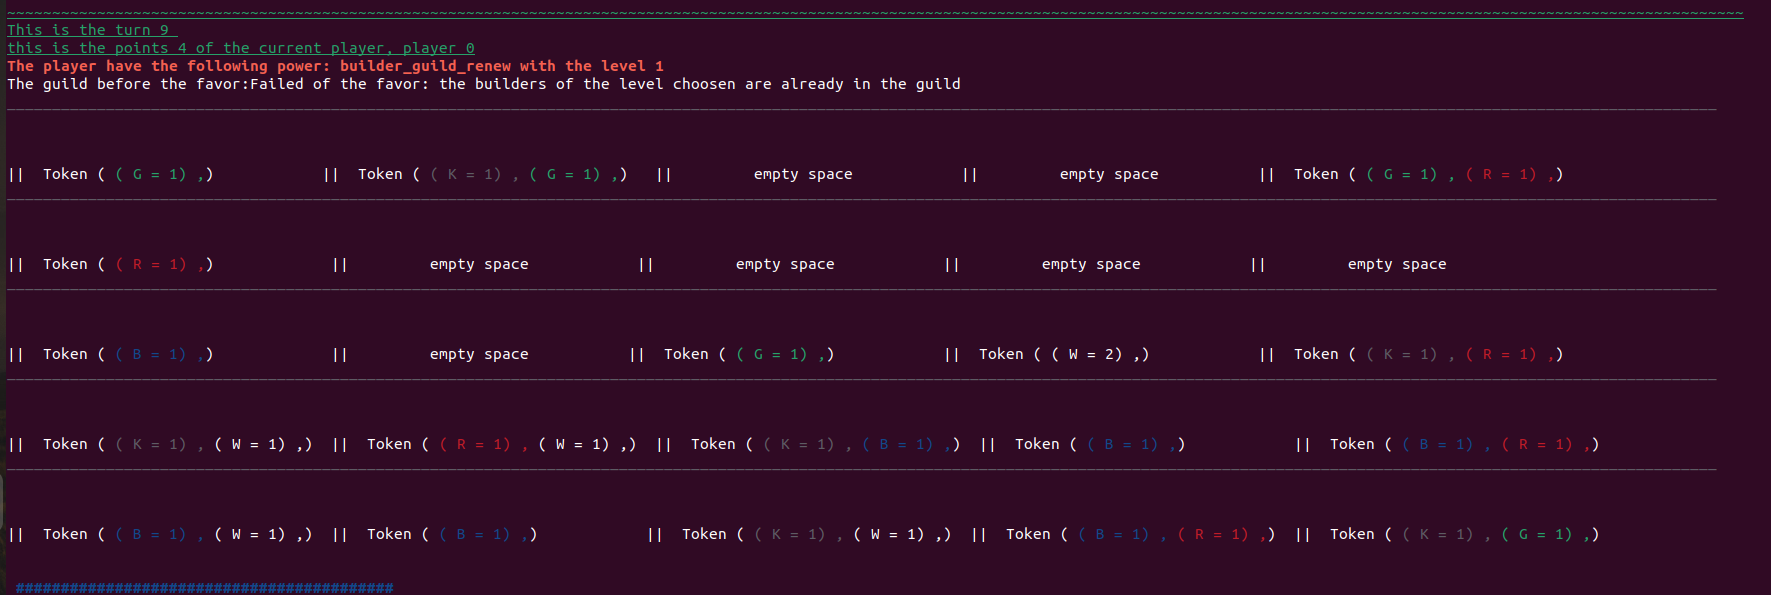
\includegraphics[width=1\linewidth]{Capture d’écran du 2024-01-12 15-39-21.png}
            \caption{Exemple explicatif de la mise à disposition des architectes}
            \label{display}
        \end{figure}

        
        \vspace{1em} De plus, ces fonctions nous ont été très utiles pour déboguer certaines parties de notre code. Par exemple, l'affichage de la guilde nous a permis de voir que le pouvoir associé (guild\_renew) était défectueux et supprimait plus d'architectes que nécessaire.
        
\section{Outils de travail}

    Lors de notre projet, nous avons appris à utiliser de nouveaux outils: que ce soit pour déboguer ou faciliter la compilation ceux-ci nous ont été extrêmement utile.
    
    \subsection{Makefile} %Expliquer comment on l'a crée et pourquoi ça nous a servi
    \hspace{1em} Pour faciliter la compilation des fichiers , on a choisi d'utiliser un Makefile, pour automatiser la compilation séparée. En effet, puisque les fichiers utilisés sont dans des sous dossiers différents, il faudrait indiquer à chaque fois les chemins relatifs lors de la création des fichiers objets, les .o. Le Makefile est constitué d'un ensemble de commande , avec les fichiers cibles associés. Pour l'exécutable "projet", qui découle de project.c, et donc de project.o, on a ajoute toutes les dépendances nécessaire à la compilation. Si le .o n'a pas été généré ou qu'il est antérieur au .c, la règle associée s'exécute à partir du .c. Ainsi un autre  avantage du makefile est qu'il ne crée les .o si et seulement s'il est inexistant ou que sa version est antérieur à celle de son .c, ce qui permet une économie de temps et de mémoire. 

    \hspace{1em} En ce qui concerne sa réalisation, nous nous sommes basés sur le Makefile donné initialement et nous l'avons étoffé, il est donc peu optimisé. Nous disposons d'une commande pour les test, qui exécute l'ensemble des tests,  une règle pour créer les fichiers .o (donné au préalable) et une commande clean, qui supprime les .o préexistants. La règle la plus importante est celle qui génère "project", avec toutes ses dépendances associées. 
    
\begin{lstlisting}[frame=single, caption={Commande de compilation},label=compilation]
project: src/project.o  src/color.o  src/token.o src/game.o src/player.o src/builder.o
src/second_builder.o src/second_token.o src/market.o src/guild.o src/stack.o 
src/permutation.o src/set.o src/super_builder.o src/super_token.o src/power.o src/favor.o
	$(CC) $(CFLAGS) $^ -o project


token: $src/token.o
	$(CC) $(CFLAGS) token.o -o token

test:tst/test.o tst/test_main.o src/color.o  src/token.o src/game.o src/player.o 
src/builder.o src/second_builder.o src/second_token.o src/set.o src/market.o src/guild.o 
src/stack.o src/permutation.o tst/test_achiev1.o src/super_builder.o src/super_token.o
src/power.o
	$(CC) $(CFLAGS) $^ -o test
	./test

\end{lstlisting} 

    \subsection{Valgrind et GDB} %Pas besoin d'expliquer réellement le fonctionnement mais on peut expliquer en quoi ça nous a servi
    \hspace{1em} Ces deux outils nous ont été utiles pour repérer les nombreuses erreurs de segmentation dûes à l'utilisation des pointeurs. Valgrind est souvent utilisé en premier recours, pour donner une idée globale de l'erreur. Une fois l'erreur repérée, on utilise gdb et grâce aux "up" et "donw" , on se déplace dans les fonctions , on peut afficher les adresses des pointeurs , ainsi que leurs contenus. Lorsque l'erreur est plus compliquée à trouver, on peut s'aider des breakpoints pour nous permettre de suivre le dérouler du code et de suivre les modifications de la valeur. Par exemple, nous avons dû faire face à une erreur de segmentation. Grâce à Valgrind, nous avons pu avoir un premier aperçu du problème, situé à priori dans notre fonction "remove\_builders\_from\_guild". Pour plus d'informations, nous avons utilisés gdb, qui nous a permis que le problème venait du fait qu'un des architectes du joueur 1 avait une adresse mémoire impossible d'accès. Nous avons rajouté un "watch player.player\_builder[i]" afin de voir à quel moment notre variable prenait la valeur interdite. Nous nous sommes ainsi aperçus que le market avait la même adresse qu'une autre structure. Cela nous a permis de nous rendre compte que cette erreur était dû à un débordement de mémoire. Nous avons choisis de créer des architectes de niveau 0, ainsi si le nombre de niveau est 2, nous avons des architectes de niveau 0 et 1, hors dans la guilde, nous avions allouer un tableau de taille [NUM\_LEVEL] pour les stacks, tout en cherchant une stack à l'indice NUM\_LEVEL (ie guild.stack[NUM\_LEVEL]). Ainsi gdb nous a permis de détecter cette erreur de dépassement de mémoire: en modifiant notre guild, on effectuait un débordement de tableau qui compromettait les valeurs situées dans cette mémoire. Néanmoins , on constate une certaine "limite" avec gdb: avec des variables globales, il est assez difficile de constater des dépassement de mémoire, au contraire de l'allocation dynamique.

    \subsection{Utilisation des tests}
     \hspace{1em} Nous avons utilisé des tests pour pouvoir valider le fonctionnement de notre code et trouver les erreurs lorsqu'elles existent.
     Nous avons notamment fait des tests pour vérifier le bon déroulement des initialisations des différentes structures. Nous avons même créé une fonction qui permet de créer un set spécifique , ce qui est pratique lorsqu'on veut vérifier le bon fonctionnement d'une fonction en particulier. 

     Il faut néanmoins reconnaître que nos tests ne sont pas exhaustifs. Nous avons privilégié d'utiliser des printf pour localiser l'erreur et de faire exécuter une partie entière plutôt que tester à petite échelle sur une partie du code.

            



    
\section{Difficultés rencontrées et solutions}
Comme dans tout travail, nous nous sommes heurté à de nombreux obstacles qui ont permis de nous forger et de nous apprendre beaucoup.

    \subsection{Les erreurs de segmentation}
    La plupart des problèmes à l'exécution résultaient d'une erreur de segmentation. Nous avons donc appris à appréhender ce type d'erreur.
    
        \subsubsection{Dépassements de tableaux}
         \hspace{1em}Comme l'illustre l'exemple précédent avec l'utilisation de gdb, nous avons fait face à de nombreuses erreurs de segmentation dûes  notamment à des dépassements de tableau dans les différentes structures de notre code."
         
        \subsubsection{Les tests de vérifications de pointeurs} %ICI énoncer le fait qu'on oubliait de mettre "if non nuLL"
        \hspace{1em} Une de nos erreurs était dûe à notre utilisation massive des pointeurs. En effet, au début, nous n'avions pas mis de barrières pour vérifier que le pointeur que nous utilisions n'était pas null. Par exemple, quand nous voulons afficher les architectes du marché, qui peuvent avoir été acheté donc peuvent être null, nous avions un problème dans le builder\_display . Nous avons donc mis des sentinelles pour éviter de travailler ou d'afficher un pointeur null.

            Pour un prochain projet, nous aimerions créer une fonction qui vérifie , dans le cas où plusieurs pointeurs pointent vers une même valeur, qu'aucun ne modifie la valeur vers laquelle ils pointent, ce qui compromettrait la cohérence du programme.
        \subsection{Erreurs en lien avec la forge} % erreur car trop de display, sol= getop() + erreur avec fichier builder.c de la forge
         \hspace{1em} Certaines erreurs ont été spécifiques à la forge, comme le fait d'avoir trop de fonctions d'affichages, ce qui engorgeait la forge et ne validait pas les tests. Pour combler ce problème, nous avons rajouté un paramètre "display", -d  à gtop, qui est de base à 0 (pour pallier à cette surcharge de display).

            Une autre erreur, plus importante cette fois-ci, est la difficulté de faire compiler notre projet, nos fichiers, avec les fichiers builder.c et token.c de la forge. L'une de nos erreurs était causée par l'assert dans la fonction "make\_builder". En effet, la fonction make\_builder du fichier de la forge, "oblige" à avoir un index inférieur ou égal à celui du nombre de builder dans la partie. Nous n'avions pas pris en compte ce paramètre, nous avions pris MAX\_BUILDER comme limite, même si le nombre d'architectes était inférieur à celui-ci. 
            
         \subsection{Implémentation des pouvoirs }
         \hspace{1em} L'implémentation des pouvoirs nous a causé quelques difficultés, notamment à cause de la cyclicité des fichiers .h inclut les uns dans les autres car le fichier power.h a besoin du fichier super\_token.h et vice versa. Pour pallier à ce problème, nous avons choisis de mettre certains .h dans les .c.

            Une autre difficulté rencontrée, est de définir un nouveau type , pour pouvoir créer un tableau des pouvoirs, qui par conséquent doivent avoir le même type. On use alors d'un typedef pour créer ce nouveau type, avec tous les arguments nécessaires à l'ensemble des fonctions, même si ces paramètres sont inutilisées dans certaines fonctions, ce qui impliquait de nombreux "warning" lors de la compilation. Pour éviter les erreurs ("warning") liés aux erreurs inutilisées, nous avons créer une macro dans le fichier power.h

            
            \begin{lstlisting}[frame=single, caption={Macro UNUSED value },label=unused]
            #define UNUSED(x) (void)(x)

    \end{lstlisting}
            
            
    
    \subsection{Exportation et manipulation de notre guilde}
        Jusqu'au milieu de notre projet, nous initialisions notre guilde dans son fichier dédié (guild.c) et toutes les modifications de la guilde se faisaient à l'aide de fonctions se trouvant dans le même fichier or les faveurs et pouvoirs nous ont amené à créer des fonctions, dans des fichiers dédié ("favor.c" et "power.c"),  qui modifiaient la guilde. Nous devions donc exporter notre guilde mais les externs étaient une mauvaise solution car ils ne rendaient pas notre code modulable pour la suite (si nous devions jouer avec 2 guildes par exemple). Nous avons donc décidé d'initialiser la guilde juste avant le début de notre guilde et de rajouter une argument de pointeur de guilde dans toutes les fonctions qui modifiaient en place précédemment la guilde. Ceci nous à montré à quel point il est important de bien rendre nos fonctions indépendantes des entités qu'elles modifient.
        
        
    \subsection{Travail de groupe}
    \hspace{1em} Le partage du travail a été compliqué initialement et au fur et à mesure s'est un peu plus équilibré. La maîtrise de git a également été laborieuse au début et , la création de branche pour pouvoir chacun avancer à notre rythme , sans écraser le code de l'autre , a été un choix judicieux pour nous. Par ailleurs, travailler avec quelqu'un , qui code différemment , a une façon de penser différente, est assez complexe. Il faut faire des concessions, accepter de déléguer, partager le travail.

    
\section{Conclusion}
 \hspace{1em} Le projet a nécessité de nombreuses compétences, techniques mais aussi humaines. Le projet nous a permis d'utiliser et de manipuler les pointeurs, de travailler avec une structure définie dans un .c, par conséquent de travailler en boîte noire. L'organisation et la répartition du travail a également été appréhendé durant ce projet.
\end{document}
